% !TeX spellcheck = en_US

\chapter{Plugin Design and Implementation}
\label{chap:ch4}
This chapter describes how the concept was implemented and presents the design of the plugin.
First, a decision had to be made, for what \gls{IDE} the extension would be implemented.
This decision, as well as some reasoning for it, can be found in \cref{sec:ch4:s1}.
Then, the icons conceived in \cref{sec:ch3:s2} needed to be created, which is described in \cref{sec:ch4:s2}.
\Cref{sec:ch4:s3} presents the architecture for the prototype.
Finally, some implementation details of the plugin, as well as interesting parts of the implementation process, are described 
and the final prototype presented in \cref{sec:ch4:s4}.

\section{Choosing the IDE}
\label{sec:ch4:s1}
The concept presented in \cref{chap:ch3} is independent of any \gls{IDE}.
However, the extension can only be implemented for one \gls{IDE} during the course of this thesis.
Therefore, a decision had to be made, which \gls{IDE} to choose.
To support this decision, the popularity, the support for creating plugins, and my prior experience were considered.

To determine the popularity, a current online ranking \footnote{\url{https://pypl.github.io/IDE.html}}, which is based on Google statistics, was consulted.
According to it, at the time of writing, Visual Studio was the most popular with a 25\% share.
The second best was \gls{Eclipse} with 16\%, followed by Android Studio and Visual Studio Code (completely separate from Visual Studio) with 11\% and 9\%.
The last two considered were pyCharm on rank 5 with 8\% and IntelliJ IDEA on rank 6 with 6\%.
We decided against Android Studio and pyCharm, as they only support the development of Android Apps and Python programs, respectively.
All the other \glspl{IDE} support multiple languages allowing the extension to be used in a more diverse set of scenarios.

Of the remaining four candidates, the ability and complexity of creating extensions were researched.
The \gls{IDE} with the easiest process to create plugins is Visual Studio Code\footnote{\url{https://code.visualstudio.com/api/get-started/your-first-extension}}.
The second best is \gls{Eclipse}, also having a lot of material helping with creating plugins for it, such as the book by Clayberg et al. \cite{clayberg2006eclipse}.
Plugins are a core concept of both and are used to provide almost all features available in these \glspl{IDE}.
Next, IntelliJ IDEA also has a fairly simple process for creating plugins\footnote{\url{https://jetbrains.org/intellij/sdk/docs/basics/getting_started.html}}.
Finally, Visual Studio also supports creating plugins, but the process is more complex than with the previous three\footnote{\url{https://docs.microsoft.com/en-us/visualstudio/extensibility/starting-to-develop-visual-studio-extensions?view=vs-2019}}.
Additionally, Visual Studio Extensions can only be developed on Windows.

\Gls{Eclipse} scored second in both of the above criteria and the winners of both categories are worse in the other.
Additionally, I already had experience with developing plugins for it.
Therefore, the \gls{Eclipse} \gls{IDE} was chosen as the one for which the extension will be implemented.

As the prototype plugin integrates the \gls{Eclipse} system into the \gls{Eclipse} \gls{IDE}, it has been named \gls{GropiusEI}.

\section{Icon Creation}
\label{sec:ch4:s2}
To create the icons described in \cref{sec:ch3:s2} the plan was made to combine multiple individual icons, one for each property, into many finished icons.
The center of each icon indicates the type of issue, as that is the most relevant property.
The main symbol's color shows the state of the issue because it is the least essential property.
However, to not discriminate people with partial or full colorblindness, a small black icon is also overlaid over the main icon.
The remaining three properties are visualized as annotations, small symbols displayed in the corners of the icon.
All of these parts are drawn as vector graphics so that the final icons can easily be scaled to any size.
One challenge while drawing was that eclipse uses 16x16 pixel icons.
Therefore, all finished icons need to convey their information even if they are just 16x16 pixels.
This significantly reduces the possible detail in the parts.

\begin{figure}[!h]
	\centering
	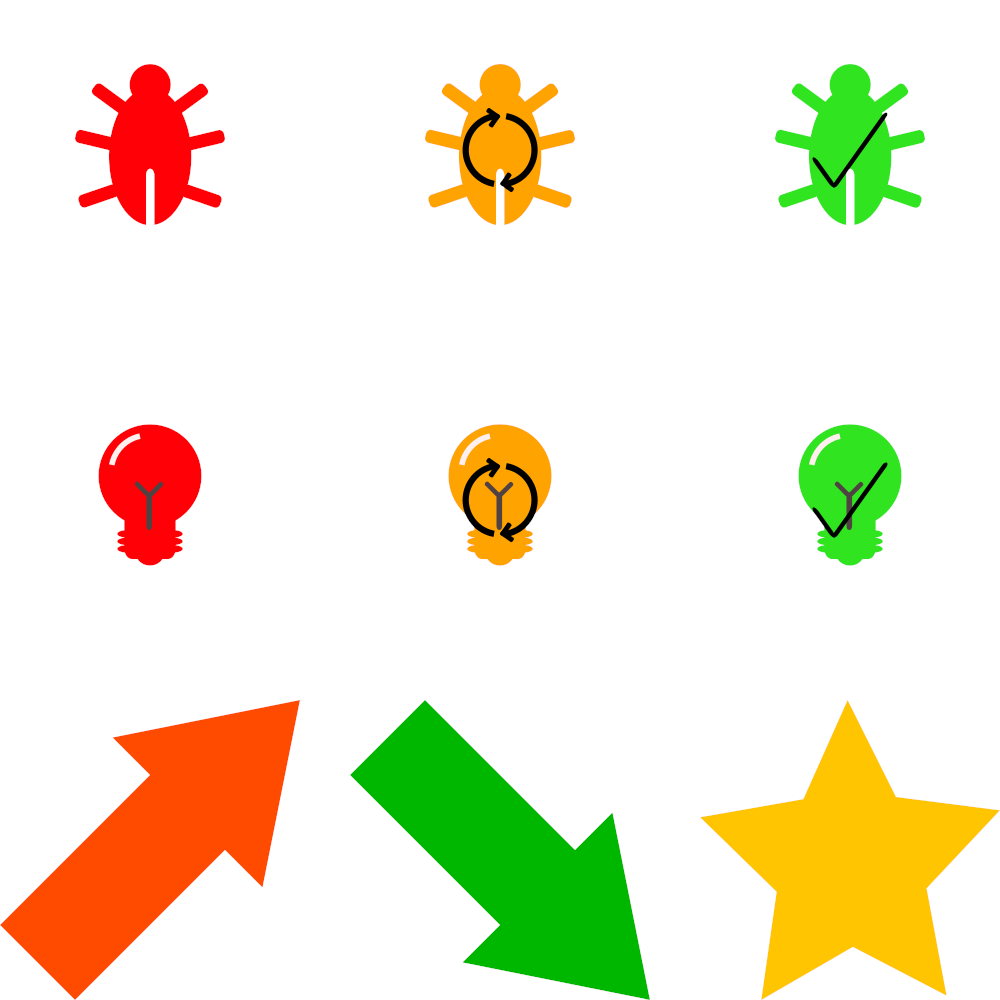
\includegraphics[width=0.5\textwidth]{graphics/iconParts.png}
	\caption{Issue Icon Parts}
	\label{fig:c4:icon_parts}
\end{figure}
\Cref{fig:c4:icon_parts} shows all the parts described above.
The first row contains the bugs in all three possible states, open, work-in-progress, and closed.
In the second row are the enhancements with the same three states.
The third row contains the annotations for the other three properties.
The first annotation is used when this issue is the cause of another issue in some other component.
In the finished icon, it is located in the top right corner.
The second symbol is the annotation for when the issue is caused by another issue and is, therefore, just a symptom of that issue.
On the final icons, this is shown in the top left.
The third symbol represents the fact that the issue is assigned to the current developer.
It is added in the bottom left of the final icon.

\begin{figure}[!h]
	\centering
	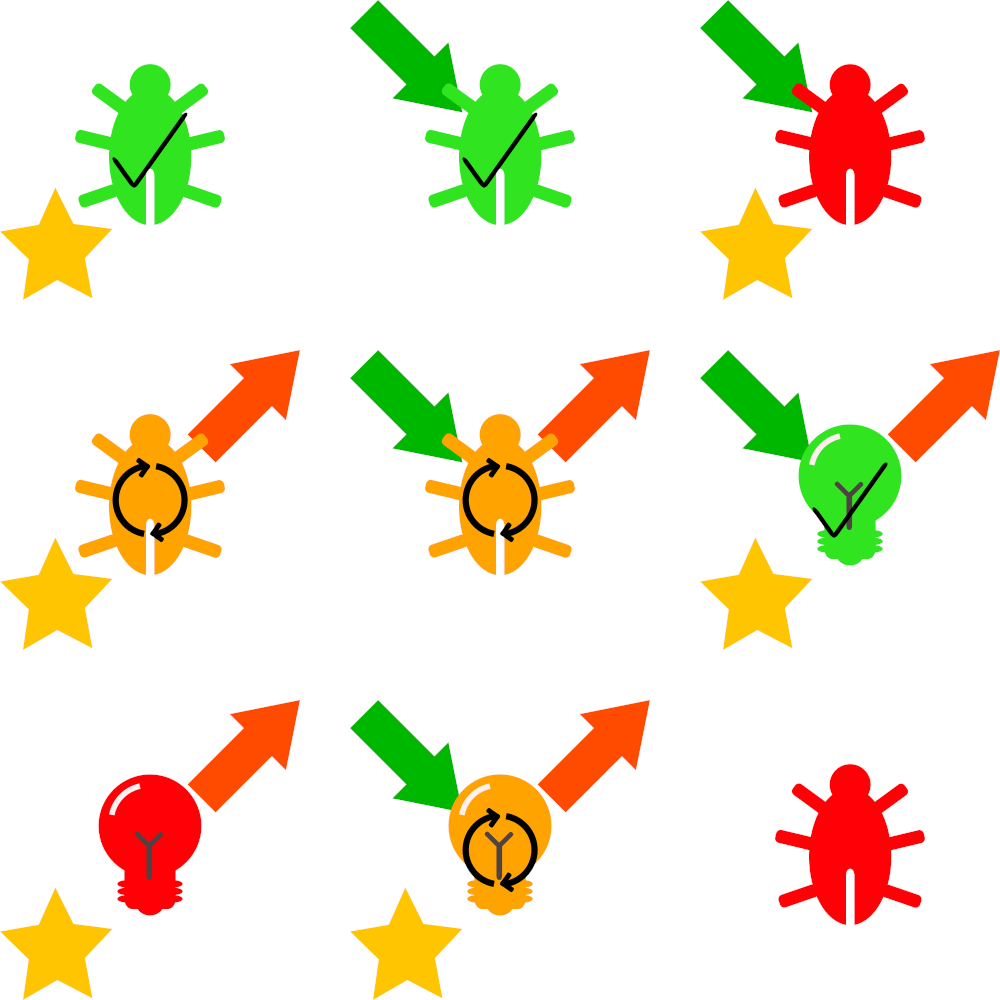
\includegraphics[width=0.5\textwidth]{graphics/iconCombinations.png}
	\caption{Issue Icon Examples}
	\label{fig:c4:icon_combinations}
\end{figure}
In \cref{fig:c4:icon_combinations} some examples of the final icons can be seen.
In total, there are 48 different combinations of the above parts.
All of those need to be created and then converted into a pixel-based image format in multiple sizes so they can be used.
This would be a very tedious manual task for one person.
Especially, as the icons were changed multiple times during the development process.
Therefore, a small script was created, which does all that automatically and results in a folder with all combinations as \gls{PNG} files in the specified sizes.

\section{Eclipse Plugin Architecture}
\label{sec:ch4:s3}
One possible approach that was investigated is to implement the plugin as an extension to Mylyn.
As described in \cref{ssec:ch2:ss2.3}, Mylyn is an \gls{Eclipse} plugin for managing tasks and can, therefore, also be used to manage plugins.
However, many of the required features from \cref{sec:ch3:s1} could, to our knowledge, not be implemented in a Mylyn extension without contributing some significant changes to Mylyn itself.
Any changes proposed for Mylyn would need to be discussed with the community and justified to the maintainers causing, in the best case, a major delay for the implementation of the extension.
In the worst case, some changes may be rejected entirely, preventing the implementation of some of the required features.
Therefore, it was decided to create a new \gls{Eclipse} extension.

As described in \cref{sec:ch3:s3}, the plugin is split into several components for portability reasons.
Therefore, the prototype actually consists of a total of four eclipse plugins, as can be seen in \cref{fig:c4:component_diagram}.
Moreover, it was decided to use a model-driven software development approach similar to the one described by Beydeda et al. \cite{beydeda2005model}.
As a big part of the tool is a list and form for viewing and manipulating data, which can be described formally,
large parts of these two \gls{UI} elements can be automatically generated that way.

\begin{figure}[!h]
	\centering
	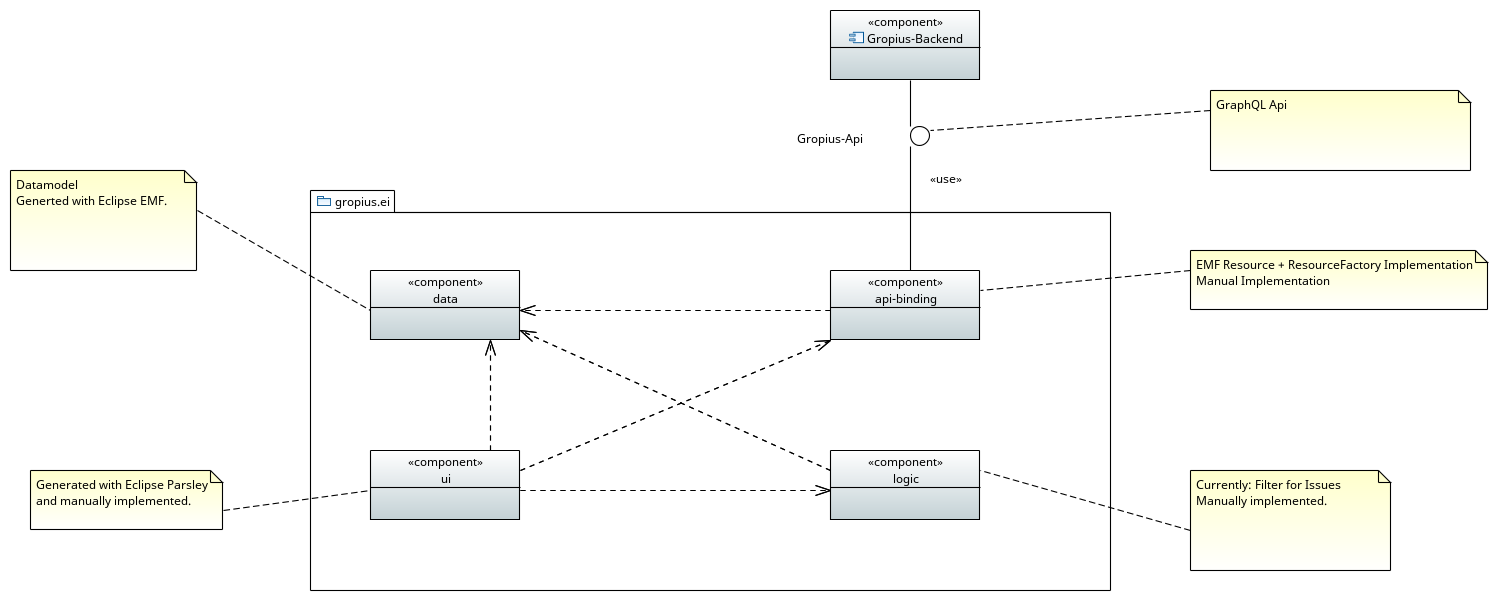
\includegraphics[width=\textwidth]{graphics/Component_Diagram.png}
	\caption{Component Diagram of the Eclipse Extension}
	\caption*{\footnotesize{The same figure can be found enlarged in \cref{chap:appendix:design_docs}}}
	\label{fig:c4:component_diagram}
\end{figure}

The plugin on the top left of \cref{fig:c4:component_diagram}, called \lstinline|data| contains the data model for the plugin. 
It is first modeled as an \gls{UML} model, then converted to an \gls{EMF} ecore model, and then the model code is generated based on that.
Ecore is the metamodel to represent models in the \gls{EMF} world \cite{steinberg2008emf}.

The plugin \lstinline|api-binding| is responsible for all communication with the \gls{Gropius} back-end through the \gls{Gropius} \gls{API}.
Additionally, it converts between the data format defined in the \lstinline|data| plugin and the format used by the \gls{API}.
As mentioned in \cref{ssec:ch2:ss1.2}, the \gls{API} provided by the Gropius system uses \gls{graphql}.
Therefore, the client needs to specify exactly what data is required and create mutations for any changes to be sent to the server.
To be able to create these mutations, the difference between the old and the new version of the change needs to be recorded.
Both the specification of the required data and the creation of mutations is also done by this component.

The third plugin, just called \lstinline|ui|, implements all the \gls{UI} elements.
It is the only plugin of the four that directly interacts with the \gls{Eclipse} \gls{IDE}.
This way, it is the only plugin, which needs major changes when the tool is ported to another \gls{IDE}, which supports Java-based plugins.
It uses the \gls{Parsley} framework introduced by Lorenzo Bettini \cite{bettini2014developing} to generate the issue list and issue details view 
based on the data model from the \lstinline|data| component.

The \lstinline|logic| plugin holds all classes containing logic needed by the \lstinline|ui|, which is not \gls{Eclipse} specific.
One example would be the classes for filtering the issues based on some properties.
They are used by the filters for the issue list but do not require any \gls{IDE} specific functions.

A separate \gls{Eclipse} plugin for the messaging component would likely make sense.
However, it was not modeled, as the idea of the messaging component was dropped from this thesis for time constraint reasons.

\begin{figure}[!h]
	\centering
	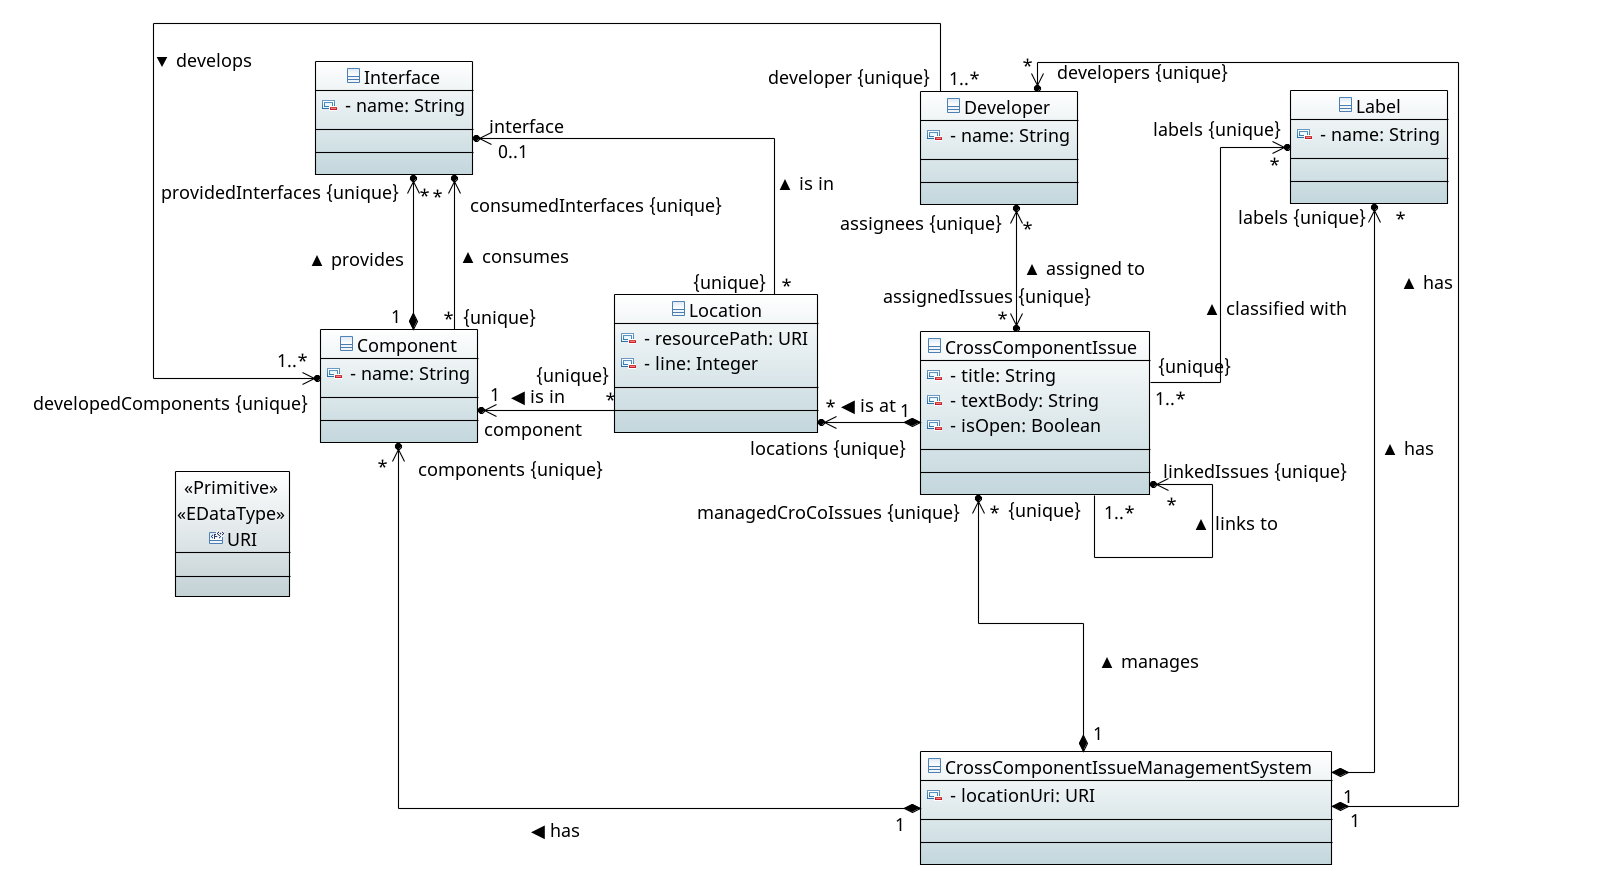
\includegraphics[width=\textwidth]{graphics/dataClassDiagram.png}
	\caption{Class Diagram of the Data Model}
	\caption*{\footnotesize{The same figure can be found enlarged in \cref{chap:appendix:design_docs}}}
	\label{fig:c4:data_class_diagram}
\end{figure}
The class diagram of the data model for \gls{GropiusEI} used to generate the \lstinline|data| component can be seen in \cref{fig:c4:data_class_diagram}.
It is based on the Domain Meta Model shown in \cref{ssec:ch2:ss1.2}.
At the core of the data model is the \lstinline|CrossComponentIssue|, with a title, text body, and a flag indicating whether it is open.
Additionally, it has various references to other objects, such as the assigned developers.

All \lstinline|CrossComponentIssue|s are contained within a \lstinline|CrossComponentIssueManagementSystem|.
That also has a list of all Labels, Developers, and Components relevant for the associated issues.
The tool always works with the issues contained in exactly one \lstinline|CrossComponentIssueManagementSystem|.

One important reference for the functionality of the tool is the \lstinline|linkedIssues| list of a \lstinline|CrossComponentIssue|.
It allows \gls{GropiusEI} to show users linked issues as well as letting users navigate between them.

Another core concept of this model are the \lstinline|Location|s.
One issue can be at zero or more \lstinline|Location|s, which specify the resource and line the \lstinline|Location| is at.
Additionally, a \lstinline|Location| can be in a \lstinline|Component| or an \lstinline|Interface|.
\lstinline|Interface|s can be provided by exactly one \lstinline|Component| and consumed by any number of them.

\section{Eclipse Plugin Implementation}
\label{sec:ch4:s4}

During the implementation phase, one of the biggest challenges was to understand and to correctly use \gls{Parsley} as well as \gls{EMF}.
Not a lot of documentation and tutorials could be found for either of them.
However, as both are open source, answers for specific questions could be searched and found in the code itself.
Yet, this process is rather tedious and slow, so a lot of time was spent just looking through these frameworks' source code.

\Gls{Parsley} is well suited for generating default \glspl{UI} for data models.
It has basic support to customize them, 
but very little existing customization already available.
Therefore, a lot of the implementation work during this thesis was improving classes, which already exist in parsley 
and adding new variants of them, which allow further customization.
Most of them could be contributed to \gls{Parsley} after a little cleanup.

\begin{figure}[!h]
	\centering
	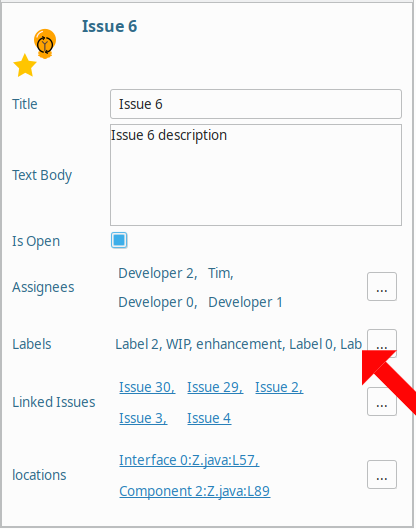
\includegraphics[width=0.5\textwidth]{graphics/screenshot_improvement_fromControl_arrow.png}
	\caption{Difference between original and new Control for Lists}
	\label{fig:c4:screenshot_improvement_formControl}
\end{figure}
One example is the \gls{UI} element displayed inside a form for the value of properties, which are lists.
Parsley only supports to display the string representation of the complete list in one label.
The new implementation of the same class allows child classes to customize this by overwriting some methods.
Based on this, some other classes were implemented using a grid of controls instead of a single label.
This allows for nicer formatting when there are too many elements for one line.
Additionally, this allows the use of links as the control for each element, which is used, for example, by the \lstinline|linkedIssues| property.
The difference between the original and the improved version can be seen in \cref{fig:c4:screenshot_improvement_formControl}.
The control for the list \lstinline|Labels| is created by the original, and you can see the last label is not entirely readable.
The other controls are the new ones, with \lstinline|Developers| using a grid of labels and the other a grid of links.

Another significant amount of time was taken by working on the \lstinline|api-binding| plugin.
As the \gls{Gropius} back-end was not ready in time, the component was implemented to work with a simple mock-up of the back-end.
Because of the fact, that the data from the \gls{API} is transformed into the data model generated with \gls{EMF}, 
the \gls{graphql} \gls{API} cannot be used as intended.
Instead, all relevant data needs to be queried at once every time the data is reloaded from the server.
This problem was detected too late to change the overall architecture of the plugin, 
mainly because the decision to switch to \gls{graphql} for the \gls{Gropius} \gls{API} was made after the concept for \gls{GropiusEI} was already done.
However, to achieve this, a complex query needs to be sent to the server.
Additionally, no appropriate \gls{java} library could be found for using \gls{graphql} \glspl{API} without manually generating the queries and manually parsing the responses. 
In the end, some open-source ruby scripts\footnote{\url{https://github.com/Shopify/graphql_java_gen}} were used to generate helper classes from the \gls{Gropius} \gls{graphql} schema.
The next problem was, that the mock-up of the back-end used to implement the \lstinline|api-binding| component is not sophisticated enough.
The returned data is not consistent in itself, preventing a correct transformation into the \gls{GropiusEI} data model.
As the real back-end would not be ready in time, the decision was made to halt implementing the \lstinline|api-binding| plugin for now.
For the remainder of the thesis, the data is generated by a mock-data generator and stored in a file instead.

\subsection{The Prototype}
Due to the lack of time, many of the features described in \cref{sec:ch3:s3} were not implemented.
Everything that was implemented is presented in the next few paragraphs.

\begin{figure}[!h]
	\centering
	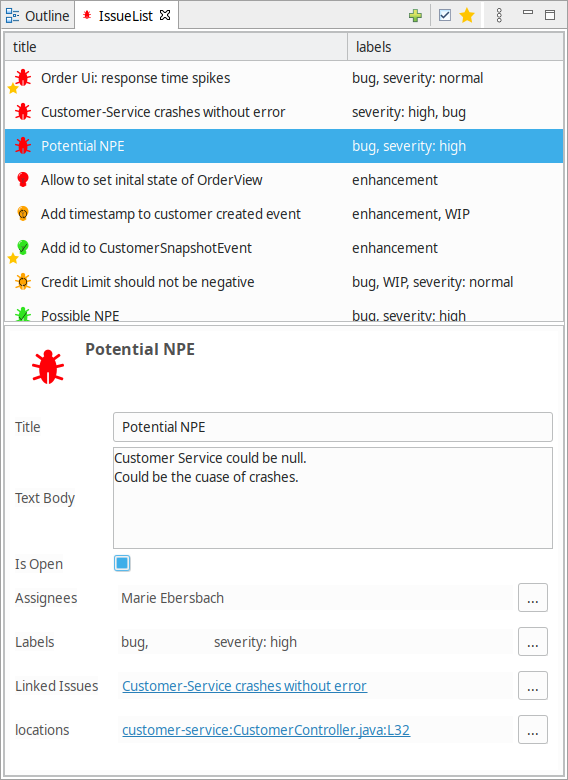
\includegraphics[width=0.45\textwidth]{graphics/screenshot_gropius_ei_issue_list.png}
	\caption{Prototype Issue List}
	\label{fig:c4:screenshot_issue_list}
\end{figure}

As stated in \cref{sec:ch3:s3} the main elements of \gls{GropiusEI} are the issue list and the issue detail view.
Deviating from the concept, those two elements are implemented in one big view element, as shown in \cref{fig:c4:screenshot_issue_list}.
This is the case because \gls{Parsley} provides such a view, and implementing interactions between the two parts is easier that way.
The issue list is in the upper half of the picture. 
It consists of multiple columns, each responsible for one property of the issues.
By default, only the title and label columns are shown, but the user can change this through the menu on the top right.
In theory, all properties that can be seen in the form in the lower half of the image can also be displayed as columns in the list.
However, especially the text body does not make much sense to be displayed in the list, as it can take a lot of space.
In the first column of the list, the icons from \ref{sec:ch4:s2} are displayed in addition to the property of that column.
Currently, the annotations for this issue being caused by another or causing another issue are not used because that feature has not yet been implemented.
The entries of columns with a list of values are not sorted in any way but display the values in the order they are contained in the respective list for this property.
This list is initially ordered by when the value was added but can be reordered by the user in the dialog for editing that property.

As you can see in \cref{fig:c4:screenshot_issue_list_filtered_sorted}, the issue list also supports sorting by a column.
This is done by clicking on the column header.
Furthermore, filtering is supported using the buttons in the bar on the top edge of the view.
Currently, only the filters \lstinline|Only show open issues| and \lstinline|Only show issues assigned to me| are implemented. 
However, all the other filters specified in \cref{sec:ch3:s3} should be fairly straight forward to include.

\begin{figure}[!h]
	\centering
	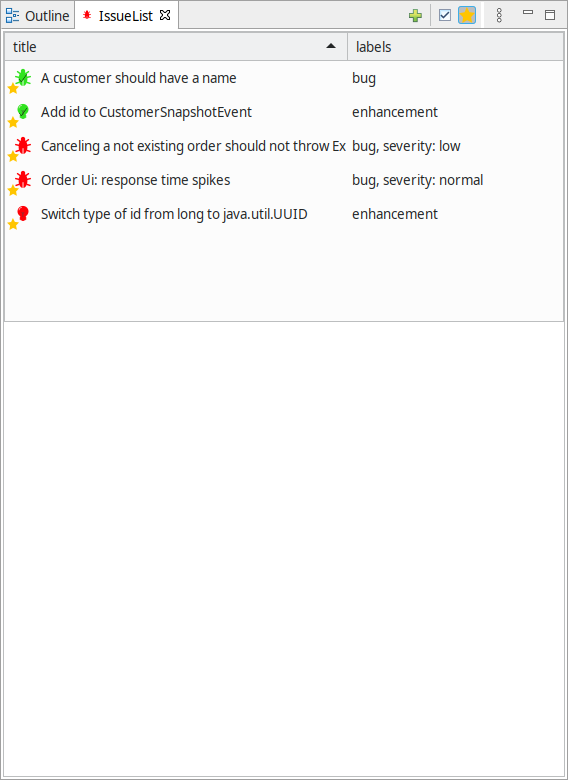
\includegraphics[width=0.45\textwidth]{graphics/screenshot_gropius_ei_issue_list_filtered_sorted.png}
	\caption{Prototype Issue List with Filter and Sorting}
	\label{fig:c4:screenshot_issue_list_filtered_sorted}
\end{figure}

\Cref{fig:c4:screenshot_issue_list} also shows the details view, which additionally is the form for editing a selected issue.
On the top of that form, the icon and the title of the issue can be seen.
Below that, all properties are displayed.
Like the issue list, the properties with multiple values are ordered according to the order in the data instead of being sorted somehow.
For the \lstinline|Linked Issues| and the \lstinline|Locations| each value is a link, 
selecting the correct issue in the list and jumping to that location in the code, respectively.
To change a textual property, the user can simply type in the corresponding text area.
The properties, which contain a list of values, can be modified using the button to the right.

\begin{figure}[!h]
	\centering
	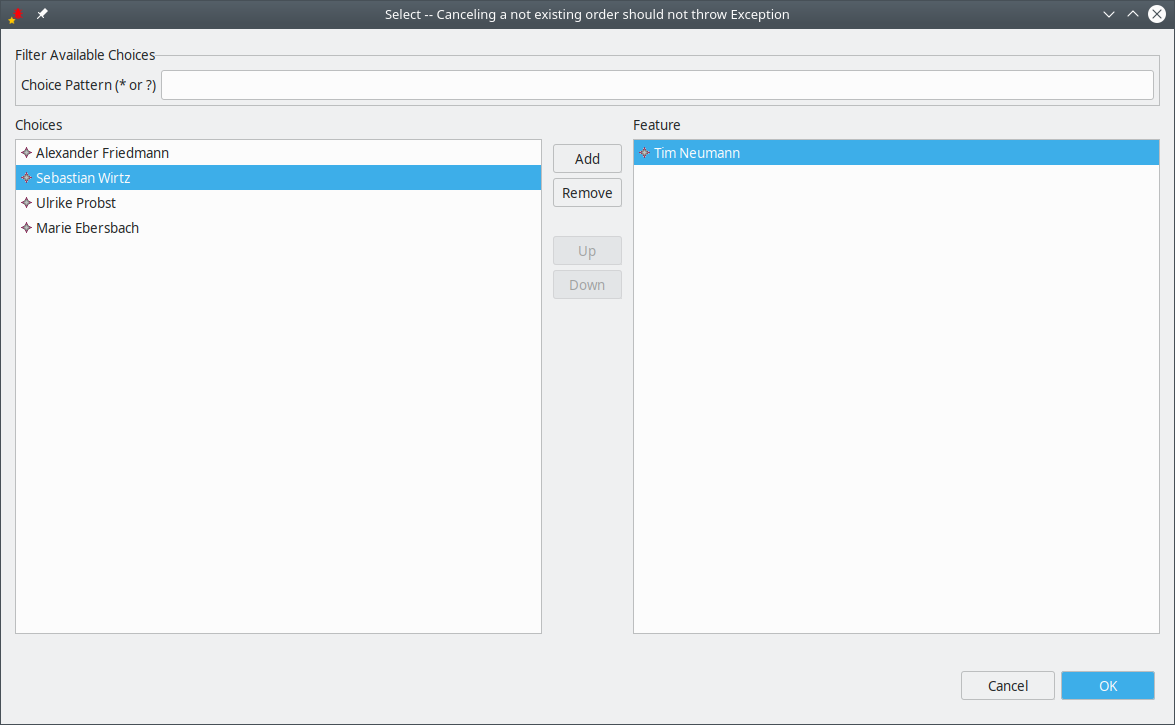
\includegraphics[width=0.8\textwidth]{graphics/screenshot_gropius_ei_edit_list.png}
	\caption{Prototype Edit Developers Dialog}
	\label{fig:c4:screenshot_edit_list}
\end{figure}

When that button is pressed a dialog similar to the one in \cref{fig:c4:screenshot_edit_list} is opened.
With it, the user can select the values for that issue from a list of all possible values for the property.
This dialog also allows the reordering of the values mentioned above.
Changes done in the dialog are applied when the \lstinline|Ok| button is pressed.

\begin{figure}[!h]
	\centering
	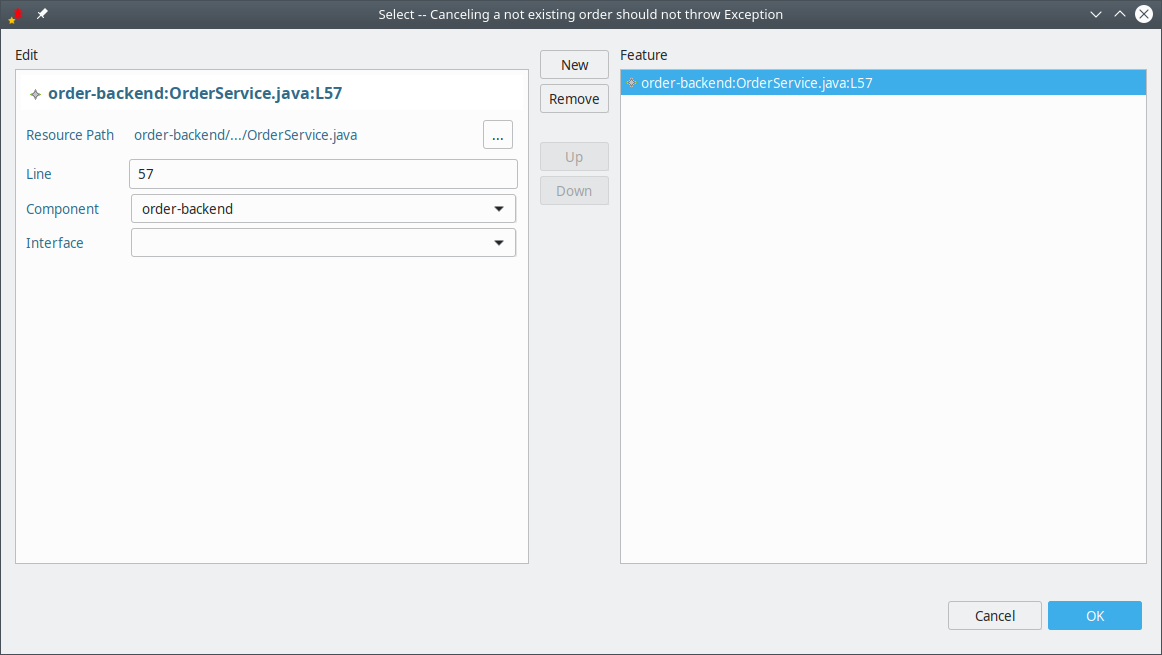
\includegraphics[width=0.8\textwidth]{graphics/screenshot_gropius_ei_edit_locations.png}
	\caption{Prototype Edit Locations Dialog}
	\label{fig:c4:screenshot_edit_locations}
\end{figure}

The only exception for the editing dialogs is the \lstinline|locations| property.
For those a dialog (shown in \cref{fig:c4:screenshot_edit_locations}), which allows creating and editing locations is opened.
Using the \lstinline|New| button, a new location is added to the list of locations for that issue.
Then it, as well as any existing location, can be edited with the left half of the dialog.

After all changes, the issue list is in an unsaved state, indicated by a star in the view name in the tab of the view.
To save the changes, all usual ways to save a resource in \gls{Eclipse} can be used, such as the save button in the toolbar.

The green plus button seen above the issue list in \cref{fig:c4:screenshot_issue_list} can be used to create new issues.
It adds a new issue with empty properties to the list, which can then be edited using the form below.
The feature for creating issues directly from some lines of code has not yet been implemented.
